\section{Evolution Propagation}
\label{sec:sec}

Everything is subject to change, and multi-model data is no exception. Changes can occur in any part of the system, such as the conceptual schema, mappings, the data itself, or the queries. When a change occurs, it is important to propagate it to all the affected components so that we can maintain consistency and correctness of the system. This process is called \term{evolution propagation}.

\todo{
    Někde zmínit migrační strategie (eager, lazy, hybrid, (predictive?)).
}

\subsection{Evolution Hierarchy}

A change in one component that is propagated to another component is also a change, so it may require further propagation, leading to a cascade of changes that can be difficult to manage. This is especially true in a multi-model data world, where there are many different components and relationships between them. This leads us to the following questions:

\question{hierarchy}{The propagation should be done in a systematic and efficient way. A change in one component should not lead (through a cascade of changes) to more changes in the same component.}

\question{hierarchy-mm}{Multi-model data naturally supports redundancy, both intra-model (i.e., some NoSQL databases promote denormalization) and inter-model (i.e., same data can be represented in multiple models). Modifications to the data in one model (or part of it) should be reflected in the other models (or parts of them) to maintain consistency.}

Our approach starts by defining a clear hierarchy of components and a set of rules for how changes should be propagated between them. On the top of the hierarchy (see \Cref{fig:evolution_hierarchy}), there is the \term{conceptual schema}. The schema can be edited via atomic operations (\acrshort{smo}s, see \paperRef{rcis_2025}), coming either directly from the user, or being automatically inferred from changes in the data (as mentioned in \Cref{sec:vision_automation}).

Next, there are \term{mappings} between the conceptual schema and the \term{logical models}. They can be edited via a subset of \acrshort{smo}s, which are automatically generated by propagating changes from the conceptual schema. They can be also created by any of the three steps from \Cref{sec:vision_automation}.

From there, changes can be propagated to the \term{data} and to the \term{queries}. The former is done via \acrshort{ddl} and \acrshort{dml} statements. Changes in data are not directly propagated back; instead, the system observes the data, infers what \acrshort{smo}s would have caused those changes, and then applies those \acrshort{smo}s to the conceptual schema and mappings.

The latter is done by directly rewriting the queries---since the queries are defined over the conceptual schema and only translated to the native database queries at execution time, they depend solely on the conceptual schema (see \paperRef{edbt_2024}). There is, again, no direct propagation from queries to other parts of the system. However, shifts in the workload (e.g., the frequency of certain queries) can be observed and used to trigger \term{self-adaptation}. Changes in query contents are not observed as the queries are considered to be dependant on the conceptual schema and not the other way around.

\begin{figure}[ht]
    \centering
    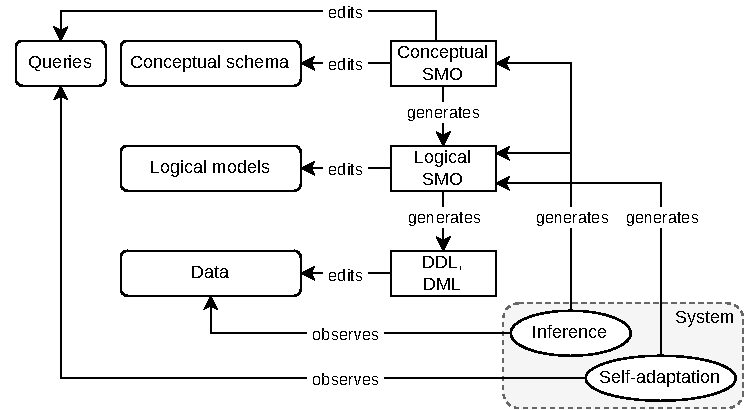
\includegraphics[width=\textwidth]{img/commentary-evolution_hierarchy.drawio.pdf}
    \caption{Hierarchy of components for evolution propagation. All changes are mediated by atomic operations (\acrshort{smo}, \acrshort{ddl}, \acrshort{dml}) and are propagated downwards. Direct changes originating outside of the system (i.e., data, query workloads) are observed and propagated upwards by inferring the corresponding atomic operations.}
    \label{fig:evolution_hierarchy}
\end{figure}

Because we use atomic operations as the basis for change propagation, we do not have to execute all of them at once. This allows us to interleave the propagation with additional user input, which is necessary for some types of operations. It also allows us to postpone the propagation until the most appropriate time, e.g., when the system is underutilized, or when the changes are expected to have the least impact on the performance of the system. By default, the data migration is done \term{eagerly}, i.e., for all data that is affected by the change. Although we did not explore \term{lazy} approaches in our research, our framework should be able to support them as well by using previous versions of conceptual schema, mappings, and queries to access the data that has not been migrated yet.

\subsection{Level of Automation}

As advertised in \Cref{sec:vision_automation}, the process of evolution propagation can be automated to different degrees. The more automation, the less manual work and expertise is required from users, but also the less control they have over the process.

\question{automation}{Very few changes can be propagated deterministically. Most of the changes require some kind of decision-making, hovewer, they should still be automated as much as possible. The user should be able to intervene the process at any point, but the system should be able to decide where to explicitly ask for user input, and where to automatically choose the best option.}

\question{query-propagation}{Propagation of changes to queries is notoriously hard, as it often requires rewriting the queries in a way that preserves their semantics, which is not always possible. Also, queries are usually written in database-specific query languages, different from languages used to model the data, therefore lacking a straightforward way to link them to the conceptual schema.}

\todo{
    Nejsem si jistý tou druhou částí této otázky, můžu to takhle napsat? Můj point je, že query v SQL nemusí být možné jednoduše namapovat na nějaké ER schéma.
}

In theory, the entire process could be fully automated with a sufficiently advanced AI system that can understand the semantics of the data and queries, predict the impact of changes, and make the best decisions about how to propagate them. In practice, we are still far from achieving this level of automation, and there are many challenges to overcome before we can get there. Therefore, we automate the process gradually following three distinct levels~\citep{ideas2022vision}.

\subsubsection{Rule-based Adaptation}

In the first level, we define the \acrshort{smo}s and their propagation rules. For example, we can use the \texttt{createProperty} operation to add an attribute \texttt{deletedAt} to an entity \texttt{Order} in the conceptual schema. This, in turn, will trigger the creation of the corresponding attribute in the logical models via the \texttt{editMapping} operation, and the addition of the attribute to the data via the corresponding \acrshort{ddl} statements.

Or, we can use the \texttt{createMapping} operation to define a new mapping to a graph model, triggering the transformation of the data from an existing relational model.

The above-described operations are deterministic and have strict preconditions and postconditions, so we can be sure that they will always lead to a consistent state of the system. However, this means there is a lot of situations that cannot be handled by the system. E.g., if an attribute is deleted and a certain query depends on it, there are several ways to rewrite the query, but none of them is strictly correct or incorrect. In such cases, a manual intervention is required to choose the preferred option. This approach was implemented in the tool \term{MM-evoque}, see \paperRef{edbt_2024} for further details.

\subsubsection{Learning-based Adaptation}

This level builds on top of the previous one by leveraging the deterministic operations and rules, but also using AI techniques to decide \emph{which} operations to apply in situations where there are multiple options. These techniques range from simple heuristics to more complex machine learning models that can learn from past examples and make informed decisions about how to propagate changes.

For example, \paperRef{rcis_2025} discusses several query propagation strategies that can be applied when an attribute is deleted, and evaluates their performance on a real-world dataset. The system can learn from the observed workload and data characteristics to choose the most appropriate strategy for each situation.

Approaches like this rely heavily on detailed insights about the workload and data. In the case of query propagation, functional dependencies between attributes are particularly useful, as they can help to identify which attributes are likely to be affected by a change and how to rewrite the queries accordingly. This is the main motivation behind the tool \term{FDepHunter}, see \paperRef{vldb_2025_fdephunter}, which is designed to not only discover functional dependencies, but also to distinguish between genuine, fake, and ghost dependencies.

\subsubsection{Self-adaptation}

Instead of reacting to changes by \uv{repairing} parts of the system whenever other parts change, the system now proactively tries to optimize its overall performance. This involve finding the right balance between the cost of and performance benefits of transforming the data to a different model, and rewriting the queries to take advantage of the new model. This is a very complex task that requires a deep understanding of the workload and data characteristics, as well as the ability to predict the impact of changes on the system's performance. These concepts are further explored in the following section.

Another form of self-adaptation is to anticipate changes before they even happen. For example, a certain set of queries might not be frequently used now, but the changes of this frequency might suggest much higher usage in the future, so the system can adapt itself in advance. This is a very ambitious goal that we are still far from achieving, but it is an exciting direction for future research.
